\documentclass{beamer}
\usepackage[english]{babel}
\usepackage[utf8]{inputenc}
\usepackage[T1]{fontenc}
\usepackage{graphicx, tikz, multicol, wrapfig}
\usepackage[framemethod=TikZ]{mdframed}


\mode<presentation>
{
    \usetheme{Boadilla}
    \usecolortheme{default}
    \usefonttheme{default}
    \setbeamertemplate{navigation symbols}{}
    \setbeamertemplate{caption}[numbered]
}


\title[Komplex viszga, ELTE 2019]{Műholdradar interferometria és GNSS mérések
                                  kombinálása 3D-s deformációs terek meghatározására}
\author[Bozsó István]{Bozsó István}
\institute[MTA CSFK GGI]{MTA CSFK Geodéziai és Geofizikai Intézet}
\date{2019.05.30.}

\def\rar{\rightarrow}
\def\lar{\leftarrow}

\newcommand\quo[1]{``#1''}
\newcommand\subt[2]{#1_{\text{#2}}}
\newcommand\pard[2]{\frac{\partial #1}{\partial #2}}
\newcommand\abs[1]{\left|#1\right|}


\newcommand\inc[1] {
    \includegraphics[width=\textwidth]{#1}
}

\newcommand\img[2] {
    \includegraphics[width=#2\textwidth]{#1}
}

\newenvironment{ffig}[1]
{
    \begin{mdframed}[linecolor=#1, linewidth=5.0pt, roundcorner=5pt,
                     innerrightmargin=10pt, innerleftmargin=10pt,
                     innertopmargin=0pt, innerbottommargin=5pt,
                     skipabove=0pt, skipbelow=0pt,
                     backgroundcolor=white, frametitle={}, align=center]
    \begin{center}
}
{
    \end{center}
    \end{mdframed}
}

\newenvironment{fig}[1]
{
    \begin{minipage}{#1\textwidth}
    \begin{center}
}
{
    \end{center}
    \end{minipage}
}


\newcommand{\fcap}[1] {
    \captionof{figure}{#1}
}

\newcommand{\genenv}[1] {
    \def\b#1 { \begin{#1} }
    \def\e#1 { \end{#1} }
}


\def\bffig { \begin{ffig} }
\def\effig {   \end{ffig} }

\def\bfig { \begin{fig} }
\def\efig {   \end{fig} }

\def\bitz { \begin{itemize} }
\def\eitz {   \end{itemize} }

\def\bmini { \begin{minipage} }
\def\emini {   \end{minipage} }

\def\bcent { \begin{center} }
\def\ecent {   \end{center} }

\def\fcol{\color{blue!55!black}}

\newcommand{\fig}[1]{
    \begin{mdframed}[linecolor=blue!65!white, linewidth=1.75pt, roundcorner=0.75pt,
                     innerrightmargin=0pt, innerleftmargin=0pt,
                     innertopmargin=0pt, innerbottommargin=0pt,
                     backgroundcolor=white, frametitle={}, align=center]
        \includegraphics[width=1.0\textwidth]{#1}
    \end{mdframed}
}

\newcommand{\figm}[2]{
    \begin{center}
    \begin{minipage}[c]{#2\textwidth}
    \begin{mdframed}[linecolor=blue!65!white, linewidth=1.75pt, roundcorner=0.75pt,
                     innerrightmargin=0pt, innerleftmargin=0pt,
                     innertopmargin=0pt, innerbottommargin=0pt,
                     backgroundcolor=white, frametitle={}, align=center]
        \includegraphics[width=1.0\textwidth]{#1}
    \end{mdframed}
    \end{minipage}
    \end{center}
}

\newenvironment{minic}[1]
{
    \begin{center}
    \begin{minipage}[c]{#1\textwidth}
}
{
    \end{minipage}
    \end{center}
}


\newenvironment{figp}[4]
{
    \begin{minipage}[c]{#3\textwidth}
    \centering
    #1
    
    #2
    \end{minipage}
    \begin{minipage}[c]{#4\textwidth}
}
{
    \end{minipage}
}


\newcommand{\figc}[2]
{
    \begin{center}
    \begin{mdframed}[linecolor=blue!65!white, linewidth=1.75pt, roundcorner=0.75pt,
                     innerrightmargin=0pt, innerleftmargin=0pt,
                     innertopmargin=0pt, innerbottommargin=0pt,
                     backgroundcolor=white, frametitle={}, align=center]
    
    \includegraphics[width=1.0\textwidth]{#1}
    \end{mdframed}
    #2
    \end{center}
}

\newcommand\sepframe[1] {
    \begin{frame}
        \begin{center}
            \Huge \fcol
            #1
        \end{center}
    \end{frame}
}


\graphicspath{{../images/}}


\begin{document}

\begin{frame}
    \titlepage
    \begin{center}
        \begin{minipage}[c]{0.3\textwidth}
            
\includegraphics[width=0.75\textwidth]{ggi_logo.png}
        \end{minipage}
    \end{center}
\end{frame}


\begin{frame}{Szintetikus Apertúrájú Radarinterferometria - InSAR}

\begin{itemize}
    \item szintetikus aprtúrájó radar - mikrohullám tartományban működő
    távérzékelési rendszer (műhold, replülő, drone)
    \item felszíni elmozdulások nagyfelbontású térképezése
    \item relatív módszer, térben, időben
    \item geodinamikai szempontból felbecsükhetetlen jelentőség, komplex
    dinamikai mintázattal rendelkező területek hosszútávú megfigyelése
    \item ESA műholdas földmegfigyelési programjában kiemelt szerep
    (Sentinel-1 A/B)
\end{itemize}

\end{frame}


\begin{frame}{InSAR korlátai}

\begin{itemize}
    \item hullámhossztól függő felszíni felbontás, 
    \item felszíni elmozdulás műholdirányú vetülete mérhető csak
    (felszálló - ascending, leszálló - descending műholdáthaladás)
    \item vegetációval sűrűn fedett területen jel koherenciája elvész
    \item visszatérési idő: 6-12 vagy több nap
    \item egyéb hullámterjedést befolyásoló tényezők szűrése: semleges
    atmoszférában, ionoszférában az EM hullám terjedési sebességének változása
\end{itemize}

\end{frame}


\begin{frame}{GGI - Űrgeodézia Kutatócsoport}

\begin{itemize}
    \item InSAR alkalmazási módjainak kiterjesztése
    \item mesterséges reflektáló pontok kifejlesztése, sarokreflektor
    \item InSAR elmozdulások kombinálása GPS mérésekkel $\rightarrow$ 3D elmozdulás
    \item jelterjedés vizsgálata, atmoszferikus, ionoszferikus hatások
    \item GGI: ionoszonda - kísérleti üzem, kísérleti eredmények
\end{itemize}

\end{frame}


\begin{frame}{GGI - Űrgeodézia Kutatócsoport}

\begin{itemize}
    \item Magyarországon: 3 sarokreflektor hálózat (Fonyód, Kulcs, Dunaszekcső)
    \item Erdélyben: 2 sarokreflektor hálózat (Parajd, Csomád);
    1 tervezett (Vrancea-zóna)
    \item eltérő felszínmozgási folyamatok (földcsuszamlás, sótektonika,
    poszt vulkáni tevékenység)
    \item ESA-PECS projekt keretérben kifejlesztett ISIGN programrendszer
    InSAR és GPS adatok kombinálására
\end{itemize}

\end{frame}


\begin{frame}{Sarokreflektorok}

\begin{center}
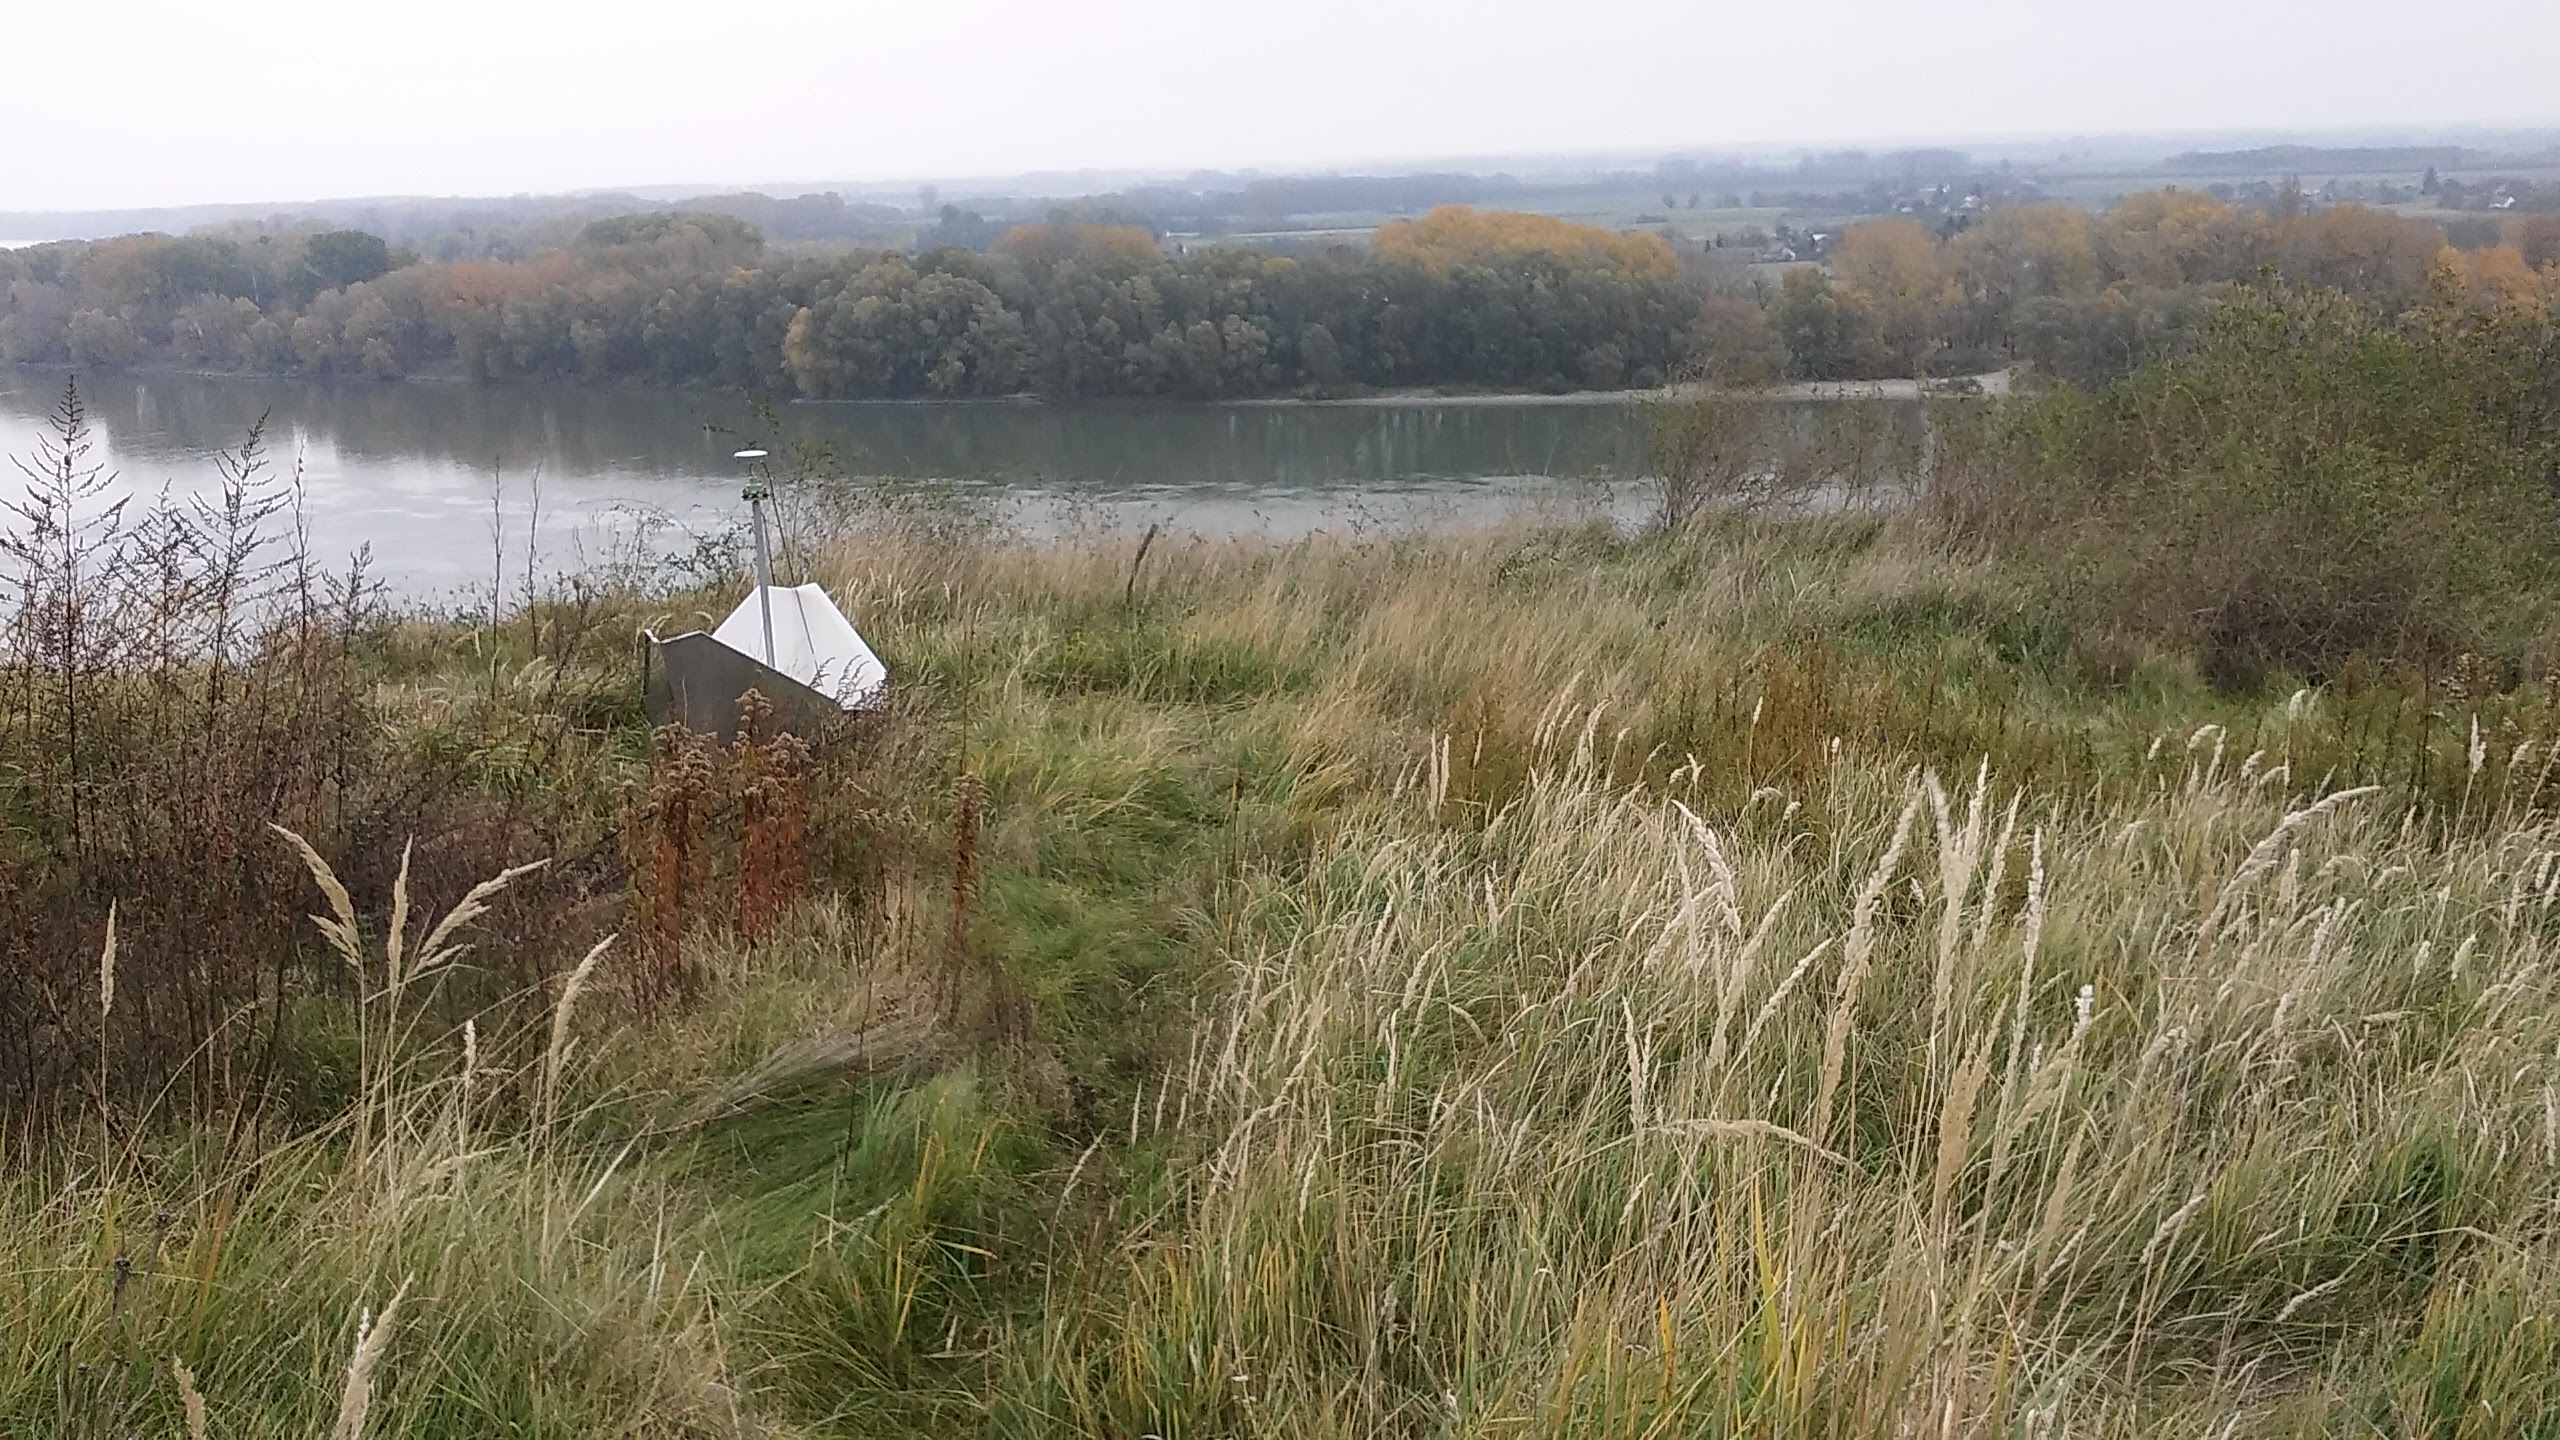
\includegraphics[width=0.75\textwidth]{dszekcso_refl_3.jpg}
\end{center}

\begin{itemize}
    \item több reflektor $\rightarrow$ reflektor hálózat
    \item elmozdulások egy kijelölt stabil referencia reflektorhoz képest
\end{itemize}

\end{frame}


\begin{frame}{Erdélyi hálózatok}
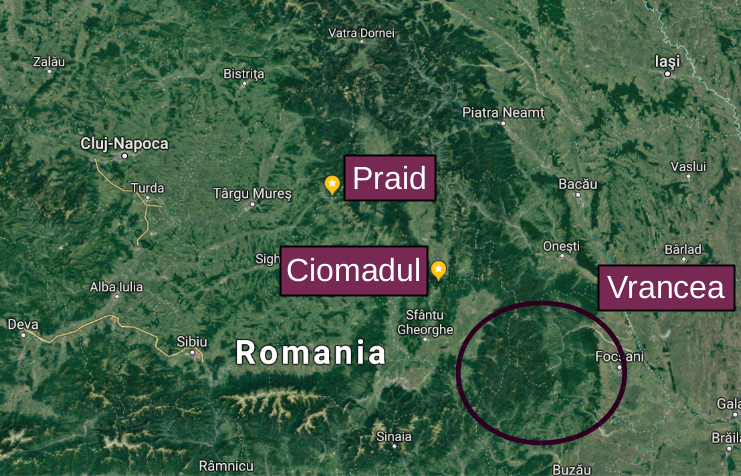
\includegraphics[width=\textwidth]{praid_ciomadul.png}
\end{frame}


\begin{frame}{Parajdi hálózat}
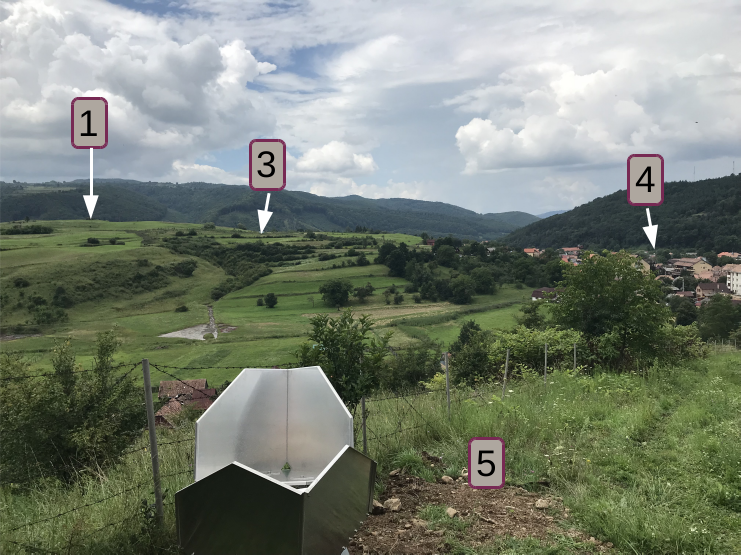
\includegraphics[width=\textwidth]{praid_refl.png}
\end{frame}


\begin{frame}{Parajdi hálózat}
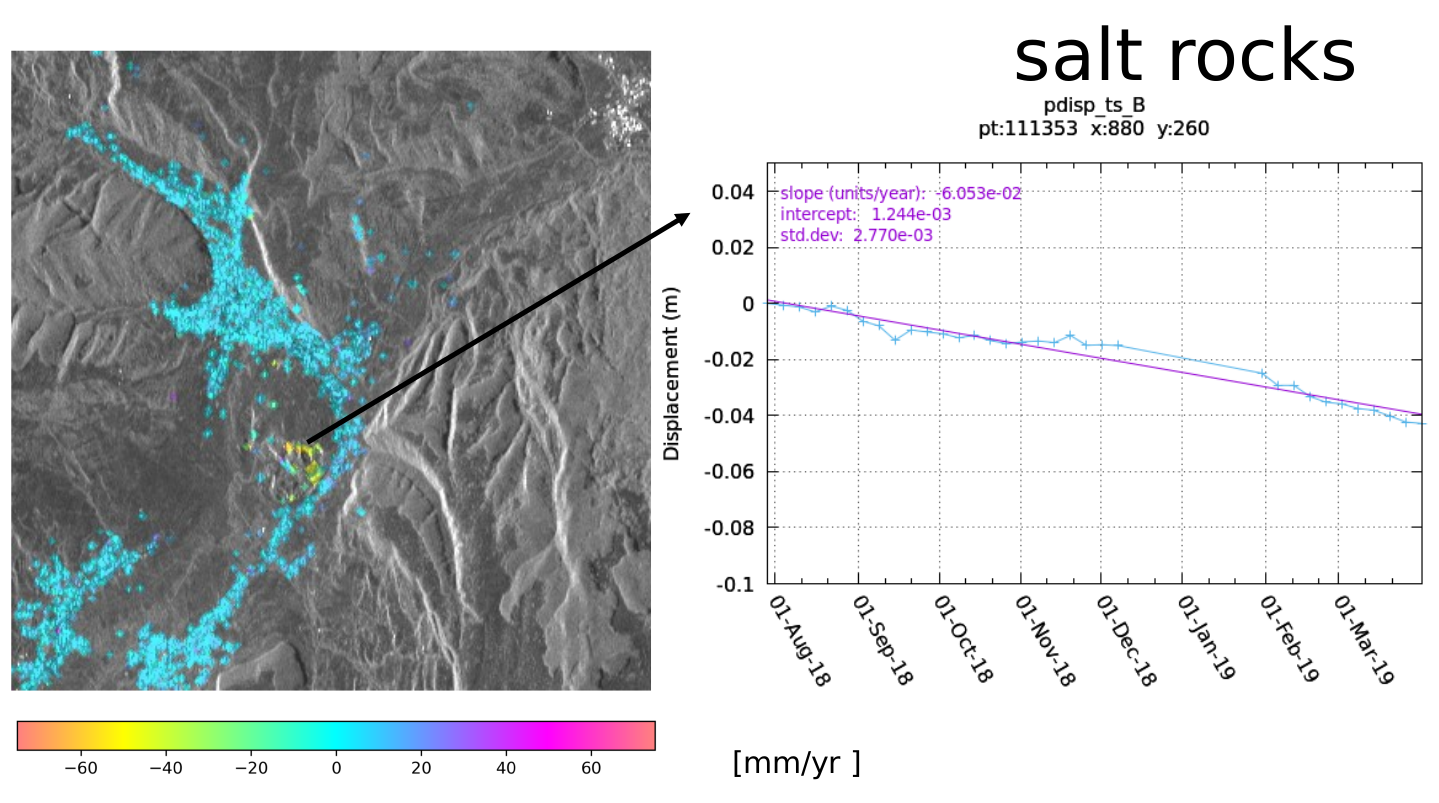
\includegraphics[width=\textwidth]{parajd_ts1.png}
\end{frame}


\begin{frame}{Parajdi hálózat}
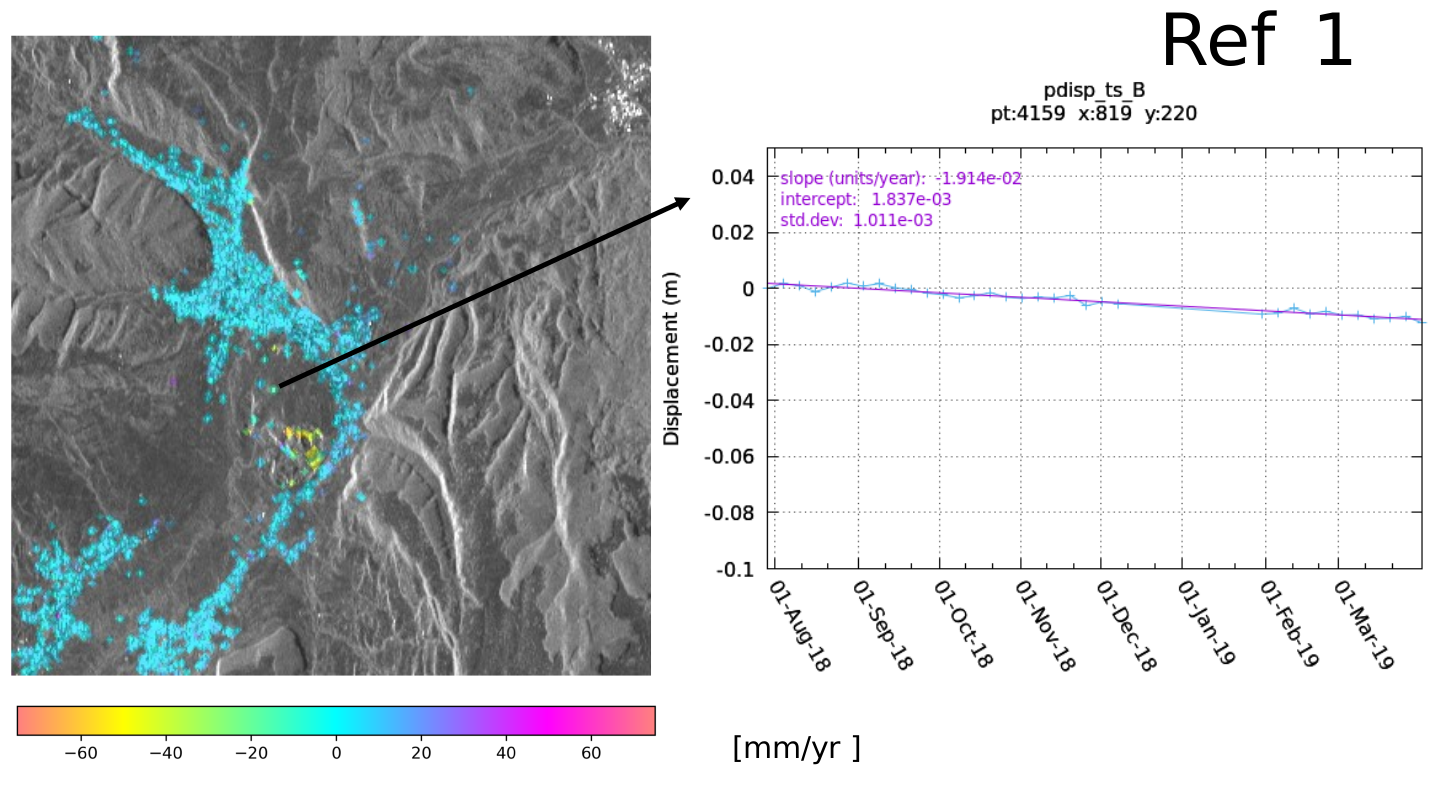
\includegraphics[width=\textwidth]{parajd_ts2.png}
\end{frame}

\begin{frame}{Parajdi hálózat}
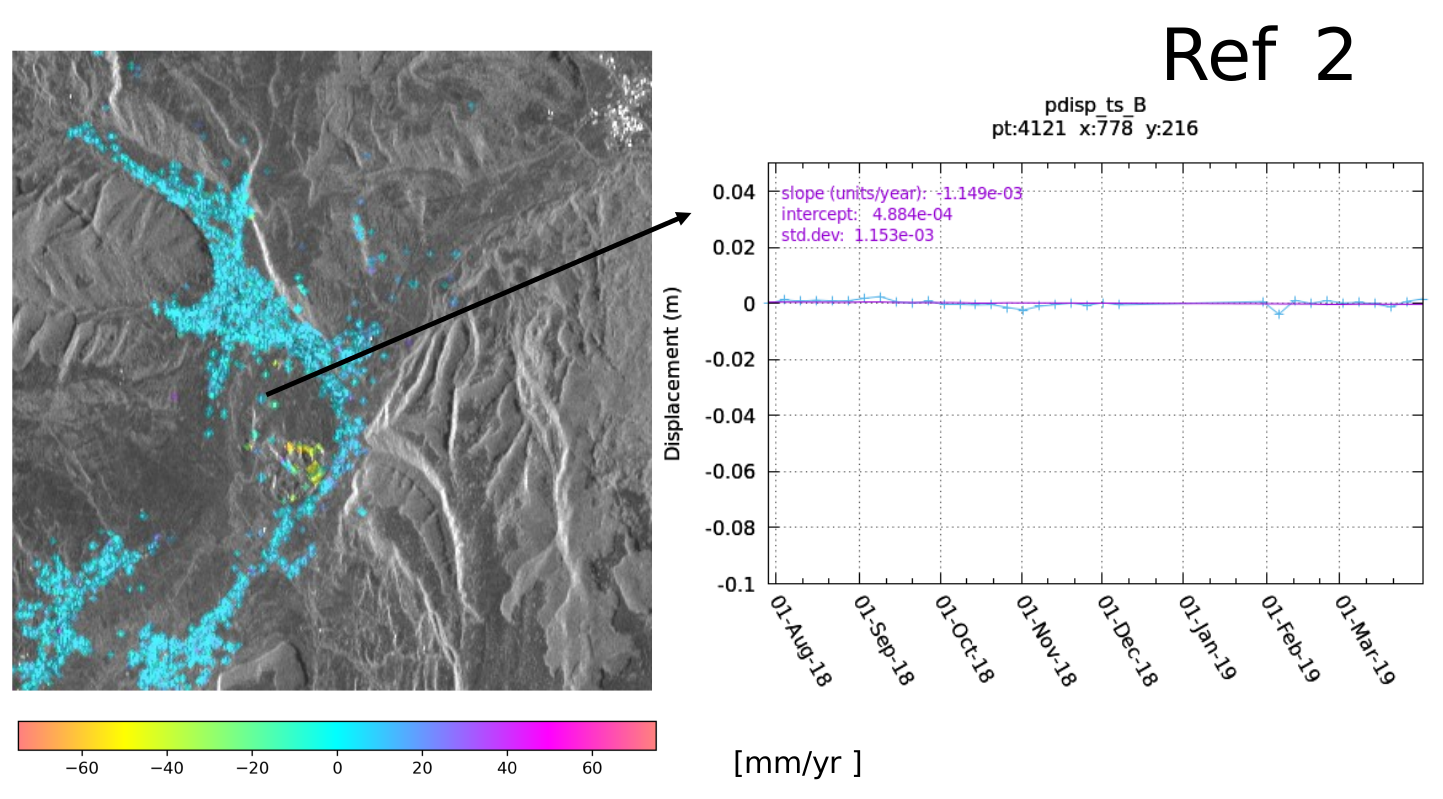
\includegraphics[width=\textwidth]{parajd_ts3.png}
\end{frame}

\begin{frame}{Parajdi hálózat}
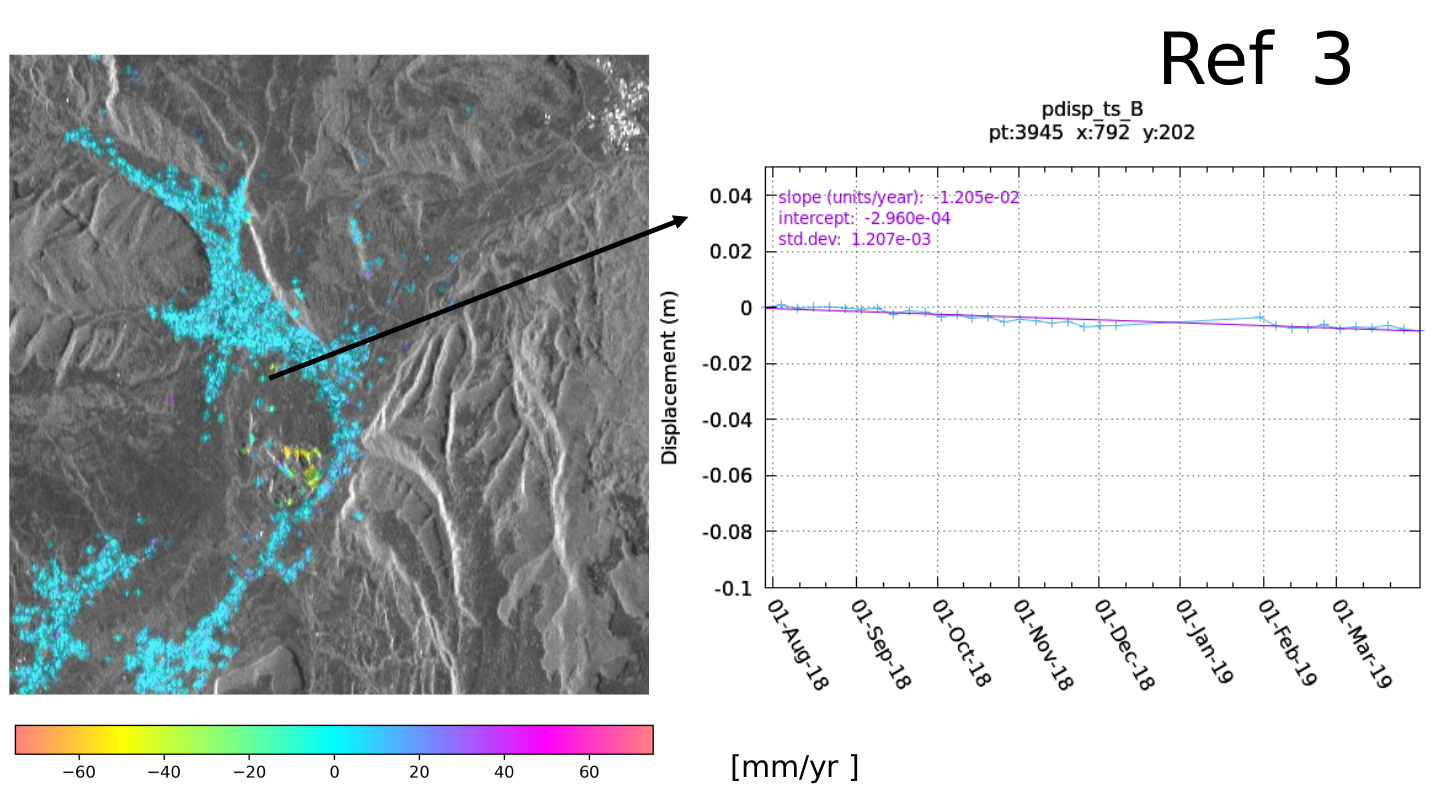
\includegraphics[width=\textwidth]{parajd_ts4.png}
\end{frame}


\begin{frame}{Magyarországi hálózatok}
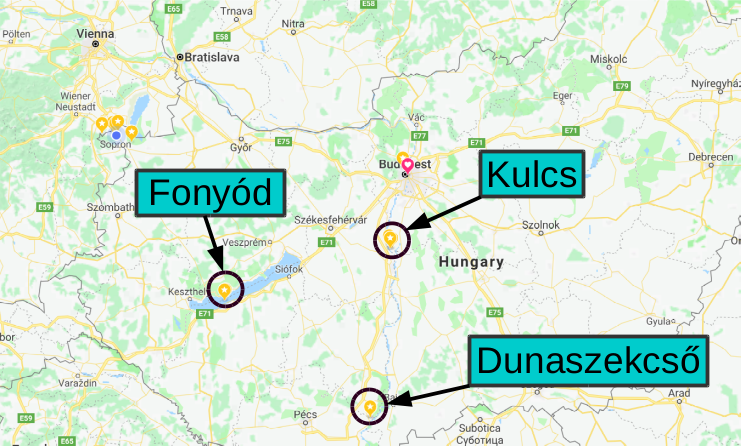
\includegraphics[width=\textwidth]{hungary_networks.png}
\end{frame}

\begin{frame}{Magyarországi hálózatok}

\begin{minipage}[c]{0.975\textwidth}
    \begin{minipage}[c]{0.475\textwidth}
        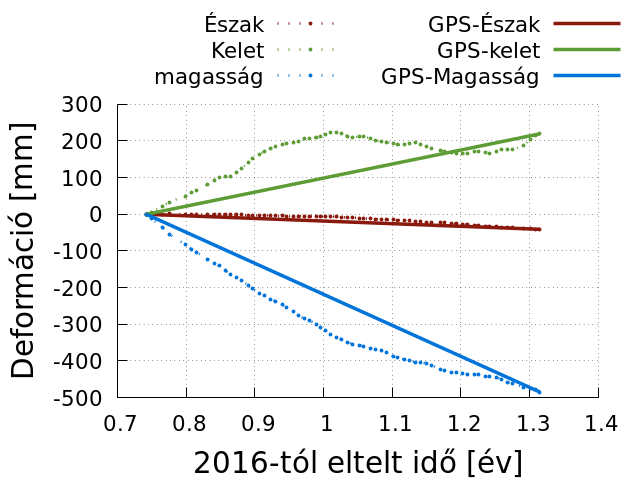
\includegraphics[width=\textwidth]{IB2-IB1_kalman.png}
    \end{minipage}
    \begin{minipage}[c]{0.475\textwidth}
        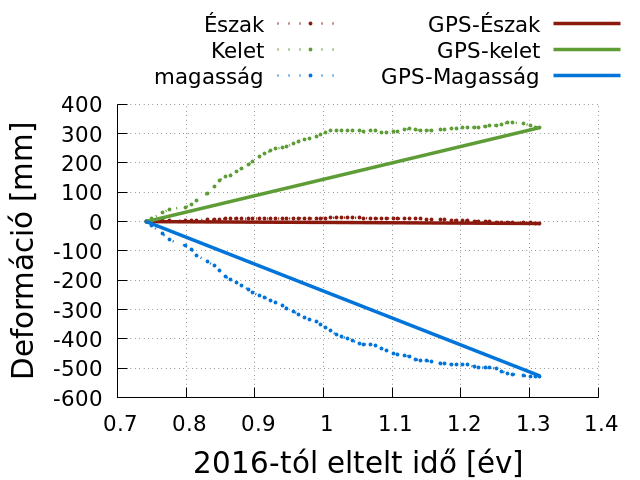
\includegraphics[width=\textwidth]{IB3-IB1_kalman.png}
    \end{minipage}
\end{minipage}
\begin{minipage}[c]{0.975\textwidth}
    \begin{minipage}[c]{0.475\textwidth}
        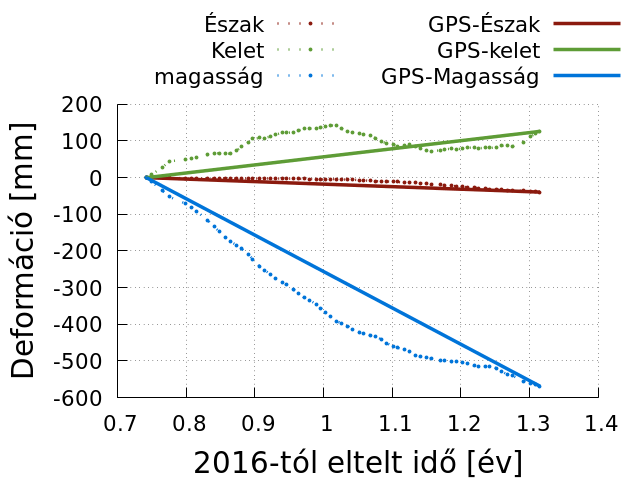
\includegraphics[width=\textwidth]{IB4-IB1_kalman.png}
    \end{minipage}
    \begin{minipage}[c]{0.475\textwidth}
        
    \end{minipage}
\end{minipage}
\end{frame}

\begin{frame}{}

\end{frame}


\begin{frame}{Integrált Vízgőzmennyiség}
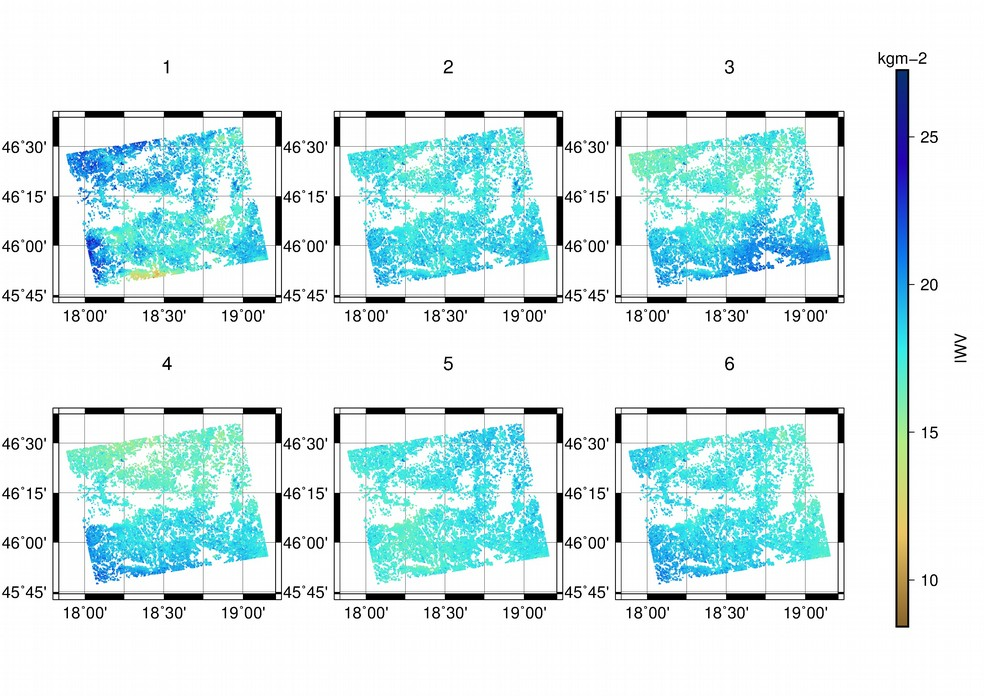
\includegraphics[width=\textwidth]{iwv.png}
\end{frame}


\begin{frame}{Integrált Elektrontartalom változás}
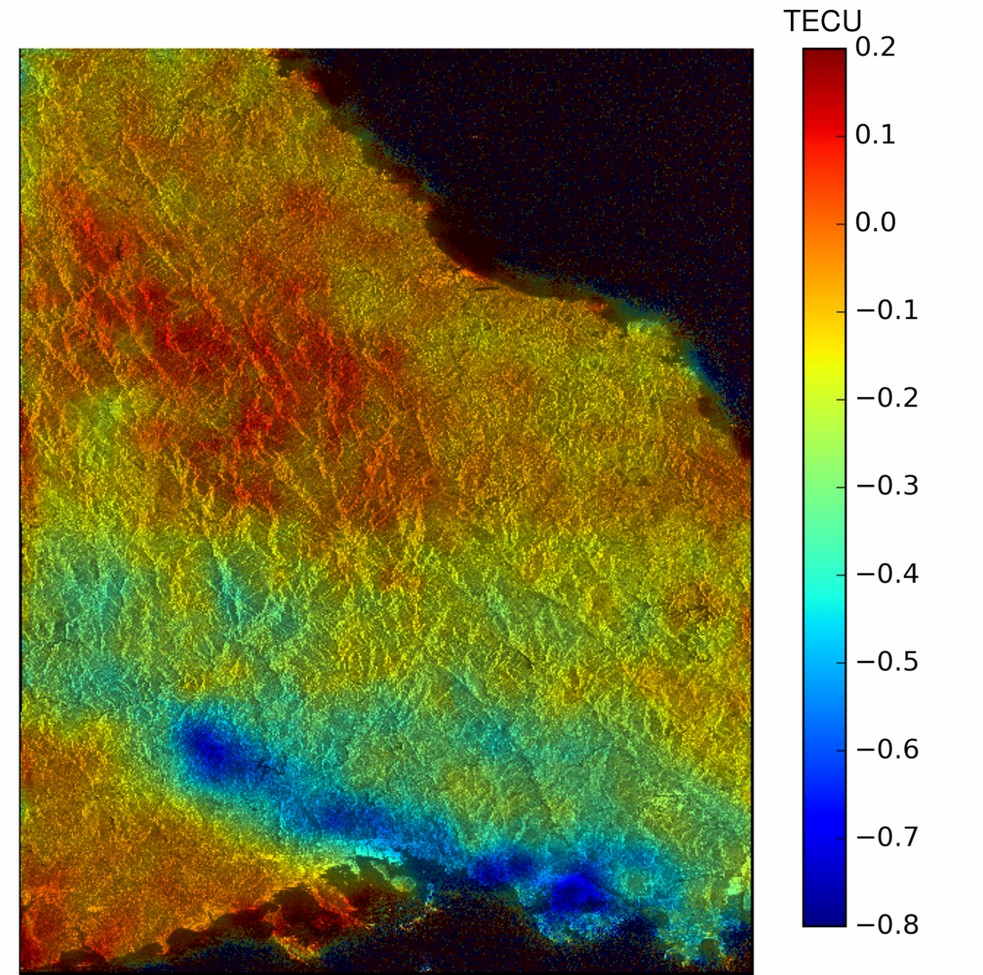
\includegraphics[width=\textwidth]{iono.png}
\end{frame}


\begin{frame}{Kutatási- és publikációs terv}

\begin{itemize}
    \item ISIGN programrendszer továbbfejlesztése, atmoszférikus
    és ionoszférikus korrekciók beépítése
    \item további reflektorhálózatok telepítése, meglévő hálózatok adatainak
    feldolgozása
    \item reflektorhálózatok feldolgozási eredményeinek publikálása
    \item nem mozgó területeken atmoszféra, ionoszféra vizsgálata
\end{itemize}

\end{frame}


\end{document}